\documentclass[12pt]{article}

% packages
\usepackage{setspace}
\usepackage{array}
\usepackage[margin=0.75in]{geometry}
\usepackage{amsmath,bm}
\usepackage{amssymb}
\usepackage{bbold}
\usepackage{physics}
\usepackage{xcolor}
\usepackage{indentfirst}
\usepackage{enumerate}
\usepackage{mathtools}
\usepackage{fancyhdr}
\usepackage{hyperref}

\newenvironment{changemargin}[2]{%
\begin{list}{}{%
\setlength{\topsep}{0pt}%
\setlength{\leftmargin}{#1}%
\setlength{\rightmargin}{#2}%
\setlength{\listparindent}{\parindent}%
\setlength{\itemindent}{\parindent}%
\setlength{\parsep}{\parskip}%
}%
\item[]}{\end{list}}

\allowdisplaybreaks

\title{Project 2: Variational Quantum Eigensolver: Constructing Potential Energy Surfaces for Small Molecules }
\date{}

\begin{document}

\maketitle

\section*{Introduction}

Currently, the Variational Quantum Eigensolver (VQE)~\cite{Peruzzo2014} 
is the most feasible technique for solving the electronic structure problem on a near-term 
noisy quantum computer. Yet, one needs to understand that VQE is a quite general framework that requires several choices to be maid by the user 
to be efficient. In what follows, we will illustrate state-of-the-art techniques to make VQE efficient for obtaining potential energy surfaces (PESs) 
for small molecules. 

A set of molecules suggested for investigation is: H$_2$, LiH, H$_4$, H$_2$O, N$_2$. They are of the increasing level of difficulty. A simple 
qualitative rule from chemistry is: the system PES is harder to calculate accurately if more chemical bonds are destroyed at the same time. 
Therefore, H$_2$ and LiH are the easiest systems (single bond), H$_4$ and H$_2$O are harder (two bonds), and N$_2$ is the hardest (triple bond).
(Actually, 1-2\% of the entire worldwide energy is spent on breaking N$_2$ bonds to make ammonia (NH$_3$) that is turned into fertilizers. 
Thus being able to model such processes is a necessary step for computational development of new catalysts for the ammonia production.)     
As a smaller correction to this qualitative picture of computational hardness, one can add a number of electrons in the system, the larger the number 
of electrons the more computationally demanding is the study. Thus, LiH is harder than H$_2$ and H$_2$O is harder than H$_4$. 

Another qualitative indicator of hardness is whether classical computing approximate methods for electronic structure that have a polynomial 
scaling are able to treat the system with chemical accuracy (1 kcal/mol). Turns out, if one breaks more than a single bond state-of-the-art approaches 
like coupled cluster single and double (CCSD) cannot achieve chemical accuracy for all points of PES. Thus, quantum computing methods based 
on VQE were thought as a viable alternative to treat such so-called strongly correlated systems.   

\subsection*{More on the topic:}

\begin{itemize}
\item Lecture 1: Electronic Structure \url{https://www.youtube.com/watch?v=0cYq9yJFYkc}
\item Lecture 2: Second Quantization \url{https://www.youtube.com/watch?v=_q4j9_D6AEg}
\item Lecture 3: Fermion-qubit Mappings \url{https://www.youtube.com/watch?v=W8SW3qp3RzY} 
\item Lecture 4:  Variational Approach \url{https://www.youtube.com/watch?v=bX5Y8mPa9oQ}
\item Lecture 5:  VQE \url{https://www.youtube.com/watch?v=UBkb54_MOLo}
\item Lecture 6:  Unitary Transformations \url{https://www.youtube.com/watch?v=981jc3Xdgvc}
\item Lecture 7:  Measurements \url{https://www.youtube.com/watch?v=U4xX5251b-E}
\item Lecture 8:  Constraints and Symmetry Projections \url{https://www.youtube.com/watch?v=mhlgldoCfx4}
\end{itemize}

\section*{Your task} \label{sec:tasks}

Using H$_2$ and H$_2$O examples, 
we will illustrate main steps of the VQE process from the setup of the Hamiltonian till obtaining the circuit for the IBM quantum computer. 
Your task will be to repeat those steps for one or two other molecules so that you can obtain the ground state PES of your molecules 
both on a classical computer using classical methods and VQE simulator, and on a quantum computer. 

Recommended bonds elongation for H$_4$ and H$_2$O are depicted in Fig.~\ref{fig:Rch}.   
Tequila is a free software package where all calculations will be illustrated.

\begin{figure}
    \begin{center}
        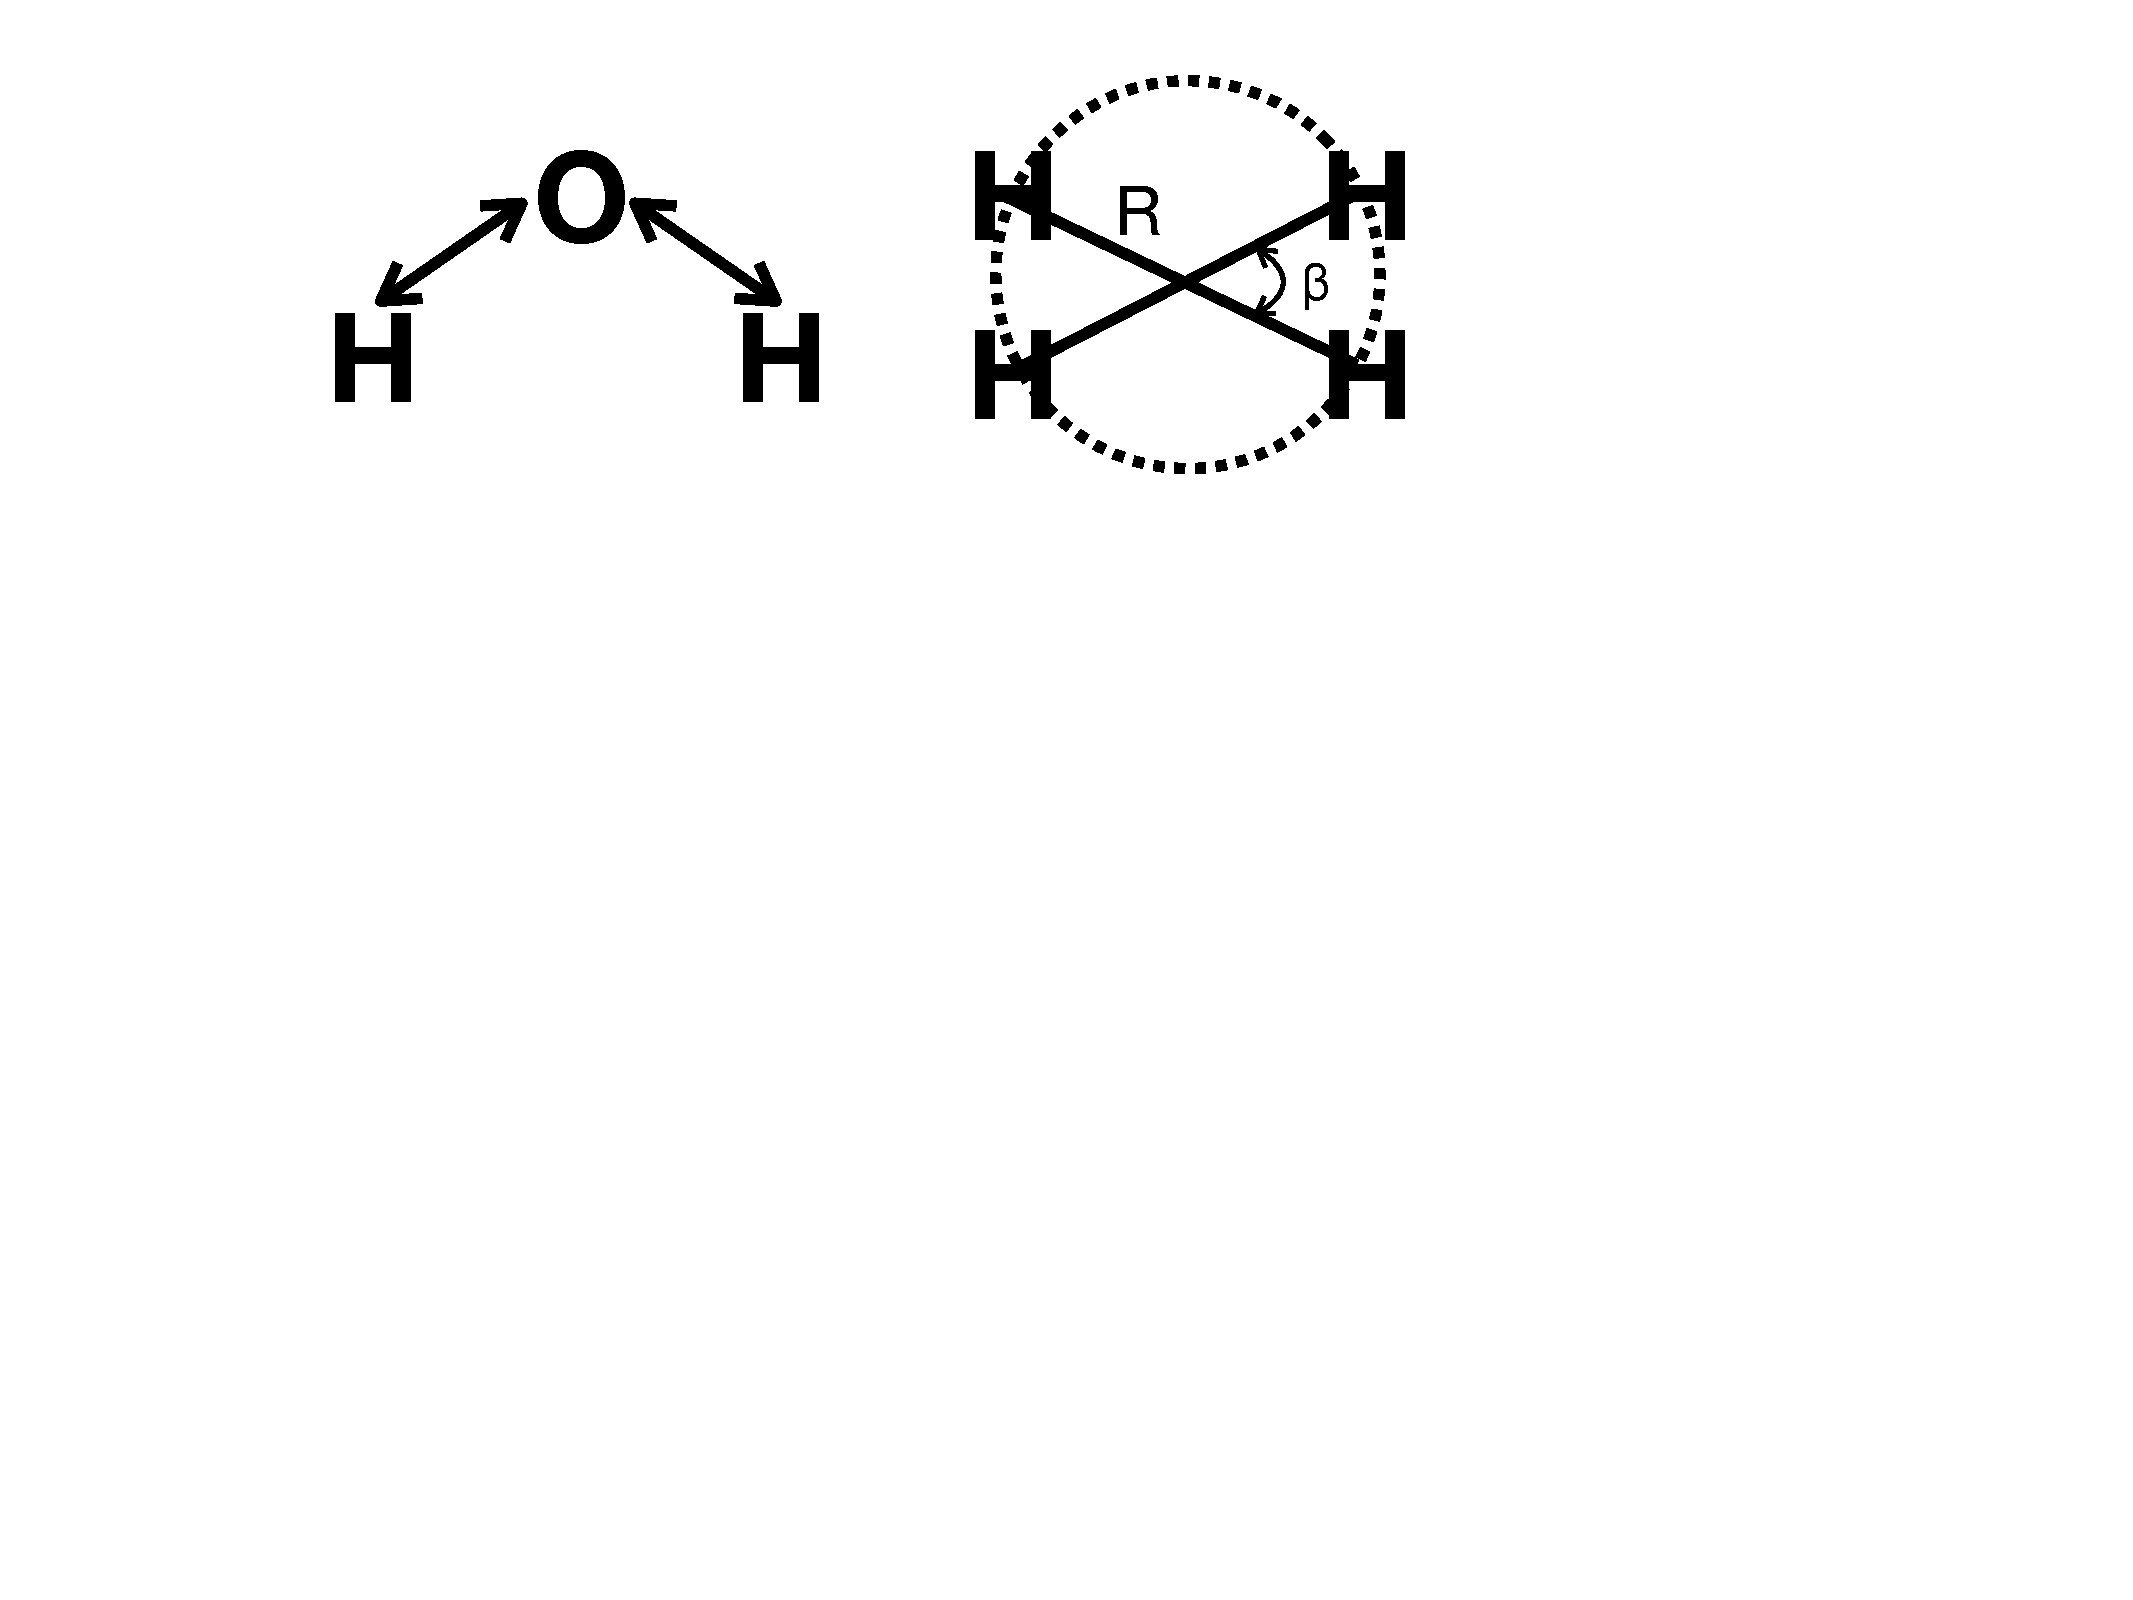
\includegraphics[width=0.5\linewidth]{Rch.pdf}
    \end{center}
    \caption{Recommended distortions: H$_2$O, symmetric OH bond length changes around $R$(O-H)=0.75 \AA~and fixed 
    $\angle$ HOH = 107.6$^\circ$; H$_4$, change of $\beta$ in the range $[85^\circ,95^\circ]$ keeping planar configuration with fixed $R$ = 1.738 \AA.}
    \label{fig:Rch}
\end{figure}

\subsubsection*{Step \#0: Setting up your computer environment}

Instructions: \texttt{S0\_Setup.pdf}.

\subsubsection*{Step \#1: Generating PES using classical methods}

Hartree-Fock (HF), Configuration Interaction Singles and Doubles (CISD), 
Coupled Cluster Singles and Doubles (CCSD), and the exact answer within the chosen basis Full Configuration Interaction (FCI)~\cite{Helgaker}.  
All these methods can easily be used for all molecules in minimal atomic basis, STO-3G. 
Comparing accuracy of PES generated for different species using different methods 
you can see the difference between weakly correlated (H$_2$, LiH) 
and strongly correlated (H$_4$,H$_2$O, N$_2$) systems. Even though the FCI method provides the exact answer it 
scales exponentially with the number of basis functions and thus cannot be used for larger systems (system size can be either correlated 
with the number of electrons or number of basis functions). All approximated methods (HF, CISD, CCSD) scale polynomially with the system 
size but fail to deliver chemical accuracy along PESs.\\

Illustrative code: \texttt{S1\_Classical\_Methods.ipynb}.

\subsubsection*{Step \#2: Generating the qubit Hamiltonian}

To proceed to VQE one needs to generate the qubit Hamiltonian, the easiest path is via first 
generating the electronic Hamiltonian in the second quantized form and then transform it into the qubit form using one of 
the fermion-to-qubit transformations: Jordan-Wigner or Bravyi-Kitaev~\cite{Seeley:2012/jcp/224109}. 
Next, some qubit operators can be substituted by numbers ($\pm 1$)
because their states are stationary for the specific electronic state (e.g. ground state). This reduction is very useful for fitting larger problem in 
a fewer qubit description and is based on Hamiltonian symmetries, which are discussed in Refs.~\cite{Bravyi:2017wba,Yen:2019bs,Setia:2019uz} \\

Illustrative code: \texttt{S2\_Hamiltonian\_gen.ipynb}.

\subsubsection*{Step \#3: Unitary transformations}

There are three main paths : 1) historically first, the unitary coupled cluster (UCC) approach has originated from the ideas of the classical 
electronic structure theory~\cite{Romero2018,Hempel2018}, 
2) hardware-efficient, direct optimization of gates and their sequence~\cite{Kandala:2017/nature/242}, 
and 3)  the qubit coupled cluster (QCC) based approach~\cite{Ryabinkin2018}. 
We will illustrate the first and third approaches, since the second one frequently runs into difficulties with energy optimization~\cite{McClean2018}. 
Among the two, even though UCC follows directly from a classical molecular orbital picture, it doesn't provide an efficient framework 
for generating gates later. In contrast, QCC can efficiently optimize energy and generate efficient circuits.

In this step, we will look at how to generate elementary unitary operations in the UCC and QCC schemes for model 
systems and to optimize their continuous parameters (amplitudes). \\ 

Illustrative code: \texttt{S3\_U\_ansatz.ipynb}.

\subsubsection*{Step \#4: Hamiltonian measurements}

To obtain the expectation value of the qubit Hamiltonian it needs to be measured at the end of the VQE circuit. 
The problem is that the entire Hamiltonian cannot be measured using current hardware. 
In this step, we show how to partition the Hamiltonian to a minimal number of groups, whose elements can be all measured simultaneously~\cite{Verteletskyi:2020do,Yen2019b}.\\ 

Illustrative code: \texttt{S4\_Measurement.ipynb}.

\subsubsection*{Step \#5: Use of quantum hardware}

To carry out the VQE algorithm on the actual quantum hardware one needs to present unitary transformations found in steps 3 and 4 as a 
sequence of gates (i.e. circuit).  Here, we will illustrate circuit generation using compilers. Obtained circuits will allow one to either carry out 
the entire VQE optimization procedure by optimizing amplitudes of step 3 unitaries or its single step using amplitudes for step 3 obtained on a 
classical simulator (easier route). \\  

Illustrative code: \texttt{S5\_Circuits.ipynb}.

\subsection*{Further Challenges} \label{sec:challenges}

Now you're on your own.  Discuss ideas for expanding on the above steps with your group.  Some possible directions for more advanced treatment:
\begin{enumerate}
\item How to obtain excited electronic states of the same or different symmetry? This task is highly relevant to any spectroscopic 
application of quantum computing because in real experiments and applications not absolute energy but their differences are measured and are important.  

\item Hamiltonian measurements (Step \#4): There are more advanced techniques to consider that are based on partitioning in the fermionic operator space and then bringing the fragments into the qubit space~\cite{huggins2019efficient,Yen:2020tt}. 

\item Unitary transformations (Step \#3): Some of the unitary transformations can be applied on the Hamiltonian instead of the wavefunction, this increases 
accuracy without increasing the circuit depth, but it increases the size of the Hamiltonian and thus introduces the measurement overhead. 
See Refs.~\cite{Ryabinkin2019b,Lang:2020uv} for details. 

\item Qubit Hamiltonian preparation (Step \#2): Typical fermion-qubit transformations substitute a single molecular spin-orbit by a qubit, which restricts calculations to relatively small basis sets because of the current limitations in the number of qubits. There were several techniques proposed recently to 
compress larger basis sets into smaller number of qubits~\cite{Takeshita:2019wn,Bauman2019b}.

\item What are alternatives to VQE for the electronic structure problem using quantum computers with shallow circuits without error-correction?
%\item Optimization of the 
  
\end{enumerate}

Business-related questions in the context of quantum entrepreneurship:

\begin{enumerate}
\item What other molecular properties one can obtain using VQE for the purpose of rational material and drug design?
\item What are the systems (molecules / materials) which are challenging for classical computing and whose modelling is valuable ?
\item What businesses can benefit from more accurate electronic structure calculations ?
\end{enumerate}

\bibliography{refs}
\bibliographystyle{unsrt}

\end{document}
